% \section{Актуальность темы}
\begin{frame}
    {Актуальность темы}
    \justifying
    В настоящее время наблюдается тенденция бурного развития процесса \textbf{«цифровизации»} нефтегазовой отрасли.
    
    % информационных технологий во всех сферах деятельности человека оказывает весомое влияние на нефтегазовый сектор страны. Соврменные компании, представляющие собой сложные многоуровневые производственные системы, для своего устойчивого развития требуют постоянного развития информационных технологий.  
    \bigskip

    % Сегодня наблюдается  бурное развитие процесса «цифровизации» нефтегазовой отрасли. 
    Одним из путей развития данного процесса является внедрение беспроводных технологий.
    \bigskip

    % Активное использование беспроводных сетей основывается на ряде их преимуществ по сравнению с кабельными сетями:
    Преимущества беспроводных сетей:
    \begin{itemize}
        \item возможность получения информации с любой точки контролируемой территории;
        \item быстрый ввод в эксплуатацию;
        \item сокращение капитальных затрат на создание сети; 
        \item уменьшение затрат на эксплуатацию;
        \item высокая гибкость, мобильность, масштабируемость;
        \item упрощенные требования к обслуживанию оборудования.
    \end{itemize}

    
\end{frame}

% \begin{frame}
%     {Актуальность темы}
%     \justifying
%     Активное использование беспроводных сетей основывается на ряде их преимуществ по сравнению с кабельными сетями:
%     \begin{itemize}
%         \item возможность получения информации с любой точки контролируемой территории;
%         \item быстрый ввод в эксплуатацию по системе подключение типа Plug-\&-Play;
%         \item сокращение капитальных затрат на создание сети; 
%         \item уменьшение затрат на эксплуатацию;
%         \item высокая гибкость, мобильность, масштабируемость;
%         \item упрощенные требования к обслуживанию оборудования.
%     \end{itemize}

% \end{frame}

% \section{Научно-техническая проблема}
\begin{frame}
    {Научно-техническая проблема}
    \justifying

    В рамках этого процесса возникает актуальная научно - техническая проблема \textbf{повышения качества проектирования беспроводной сети связи}, осуществляющей сбор и передачу информации в центр  управления с множества контролируемых объектов на некоторой территории. 

\end{frame}


\begin{frame}
    {Научно-техническая проблема}
    Процесс проектирования БШС состоит из последовательного решения взаимосвязанных задач:
    
    \bigskip

    \begin{itemize}
        \item выбор типов технических средств и протоколов;
        \item \textbf{выбор топологической структуры сети;}
        \item анализ и оптимизация пропускной способности каналов связи, маршрутизация информационных потоков и т.д.
    \end{itemize}

    \bigskip
    
    Задача \textbf{синтеза топологии} при комплексном проектировании БШС является основной проблемой исследования в данной работе.

\end{frame}

\begin{frame}
    {Научно-техническая проблема}

    \textbf{\underline{Объектом исследования}} БШС специальных типов, широко представленных на практике:
    
    \bigskip

    \begin{itemize}
        \item БШС для контроля линейных траекторий;
        \item БШС с ячеистой топологией (mesh) для контроля объектов, рассредоточенных на некоторой территории.
    \end{itemize}

    \bigskip

    \textbf{\underline{Предметом исследования}} является синтез топологической структуры беспроводной широкополосной сети.

    \bigskip
    
    \textbf{\underline{Целью}} является разработка моделей и методов оптимального размещения базовых станций для БШС указанных типов, определяющего топологию таких сетей.
\end{frame}

% \section{Положение 1, 2, 3}
\begin{frame}
    \justifying
    \begin{center}
        {\textbf{Положение 1} - математические модели в виде задачи ЦЛП и экстремальной комбинаторной задачи для оптимального размещения базовых станций при проектировании БШС с линейной топологией;}
        \bigskip
        
        {\textbf{Положение 2} - специальный алгоритм МВ и Г для решения сформулированной
        экстремальной комбинаторной задачи;}
        \bigskip

        {\textbf{Положение 3} - итерационная процедура нахождения последовательности лучших
        решений для задачи размещения базовых станций в рамках комплексного
        проектирования БШС с линейной топологие.}
    \end{center}
\end{frame}

\begin{frame}
    {Технологическая постановка задачи} 
    \justifying
    Для контроля над заданным линейным участком необходимо разместить базовые приемопередающие устройства (станции) таким образом, чтобы максимизировать покрытие с обеспечением условий технических и бюджетных ограничений. 

    \bigskip
    
    Постановка
    \begin{itemize}
        \item в виде задачи ЦЛП;
        \item в виде комбинаторной модели в экстремальной форме.
    \end{itemize}

\end{frame}

% \begin{frame}
%     Важно обеспечить связь любой станции со шлюзами на концах участка через систему размещенных станций. Задано множество станций
% \end{frame}

\begin{frame}
    {задача ЦЛП}
    \justifying
    % Задаче в виде ЦЛП формулируется следующим образом. 

    \bigskip

    Задано множество станций $S = \{s_j\}$. Каждой станции приписаны параметры $s_j = \{r_j, \{R_{jq}\}, c_j \}$, $j = \overline{1,m}; q = \overline{1,m}; q \neq j$. 
    \begin{itemize}
        \item $r_j$ -- радиус покрытия станции,
        \item $R_{jq}$ -- радиус связи между станцями $s_j$ и $s_q$,
        \item $c_j$ -- это стоимость.
    \end{itemize} 
    
    \bigskip

    Задан линейный участок длиной $L$ с концами в точка $a_0$ и $a_{n+1}$. 
    
    Внутри  отрезка $[a_0, a_{n+1}]$ задано конечное множество точек $A=\{a_i\}, i=\overline{1,n}$; эти точки соответствуют набору свободных мест, где могут быть размещены станции.
    
    Каждая точка $a_i$ определяется своей одномерной координатой $l_i$. 
    
    \bigskip
    
    Заданы станции специального вида $s_{m+1}$ -- шлюзы. Данные шлюзы размещены на концах $a_0$ и $a_{n+1}$ данного линейного участка. 
    \bigskip

\end{frame}

\begin{frame}
    {задача ЦЛП}
    \begin{minipage}[t]{1\linewidth}
        \fontsize{8pt}{7.2}\selectfont
        \justifying
        Уравнение энергетического потенциала канала связи:
        $$
        P_{tr} - L_{tr} + G_{tr} - L_{fs} + G_{recv} - L_{recv} = SOM + P_{recv},
        $$
        где: $P_{tr}$ -- мощность передатчика, дБм; $L_{tr}$ -- потери сигнала на антенном кабеле и разъемах передающего тракта, дБ; $G_{tr}$ -- усиление антенны передатчика, дБ; $L_{fs}$ -- потери в свободном пространстве, дБ; $G_{recv}$ -- усиление антенны приемника, дБ; $L_{recv}$ -- потери сигнала на антенном кабеле и разъемах приемного тракта, дБ; $SOM$ -- запас на замирание сигнала, дБ; $P_{recv}$ -- чувствительность приемника, дБм.

        \bigskip
        Формула Фрииса, выраженная в децибеллах:
        $$
        \label{eq:part3_L_fs}
        L_{fs} = 20 \lg{F} + 20\lg{R} + K,
        $$
        где $F$ -- центральная частота, на котором работает канал связи, $R$ -- рассточние между приемной и передающей антенной и $K$ -- константа, зависящая от размерностей частоты и расстояния:
        
        \bigskip
        Радиус связи $R_{jq}$  и радиус покрытия $r_j$ рассчитывается как

        $$
        R_{jq} / r_j = 10^{\left(\frac{L_{fs} - 20\lg{F} - K}{20}\right)}.
        $$
    \end{minipage}

\end{frame}


\begin{frame}
    \frametitle{задача ЦЛП}
    \begin{minipage}[t]{1\linewidth}
        \fontsize{8pt}{7.2}\selectfont
        Целевая функция:
        \begin{equation}
        f =  \sum\limits_{i=1}^n (y_i^- + y_i^+) \rightarrow max,
        \end{equation}

        где $y_i^+$ и $y_i^-$ , $i= \overline{0,n+1}$ определяют охват покрытия (справа и слева, соответственно) станций.
        \bigskip
    \end{minipage}

    \begin{minipage}[t]{0.5\linewidth} 
        \fontsize{8pt}{7.2}\selectfont
        Каждая станция должна быть размещена только в одной точке:
            
        \begin{equation}
        \label{eq:part3_xij}
        \sum\limits_{j=1}^n x_{ij} \leq 1, \quad j = \overline{1,m}. 
        \end{equation}
        
        % Значения покрытий не превышают радиус покрытия станции, размещенной в точке $ a_i $, и равны 0, если в точке $a_i$  нет станции \cref{eq:part3_yi_1, eq:part3_yi_2}:
        
        
        \begin{equation}
        \label{eq:part3_yi_1}
        y_i^+ \leq \sum\limits_{j=1}^m x_{ij} \cdot r_j, \quad i = \overline{1,n};
        \end{equation}
        
        \begin{equation}
        \label{eq:part3_yi_2}
        y_i^- \leq \sum\limits_{j=1}^m x_{ij} \cdot r_j, \quad i = \overline{1,n}. 
        \end{equation}

        $$
            x_{ij} = 
             \begin{cases}
               1& \text{, станция $s_j$, размещенная на точке $a_i$,} \\
               0 & \text{, в противном случае.}
             \end{cases}
        $$

    \end{minipage}
    \hfill
    \begin{minipage}[t]{0.4\linewidth}
        
        \center{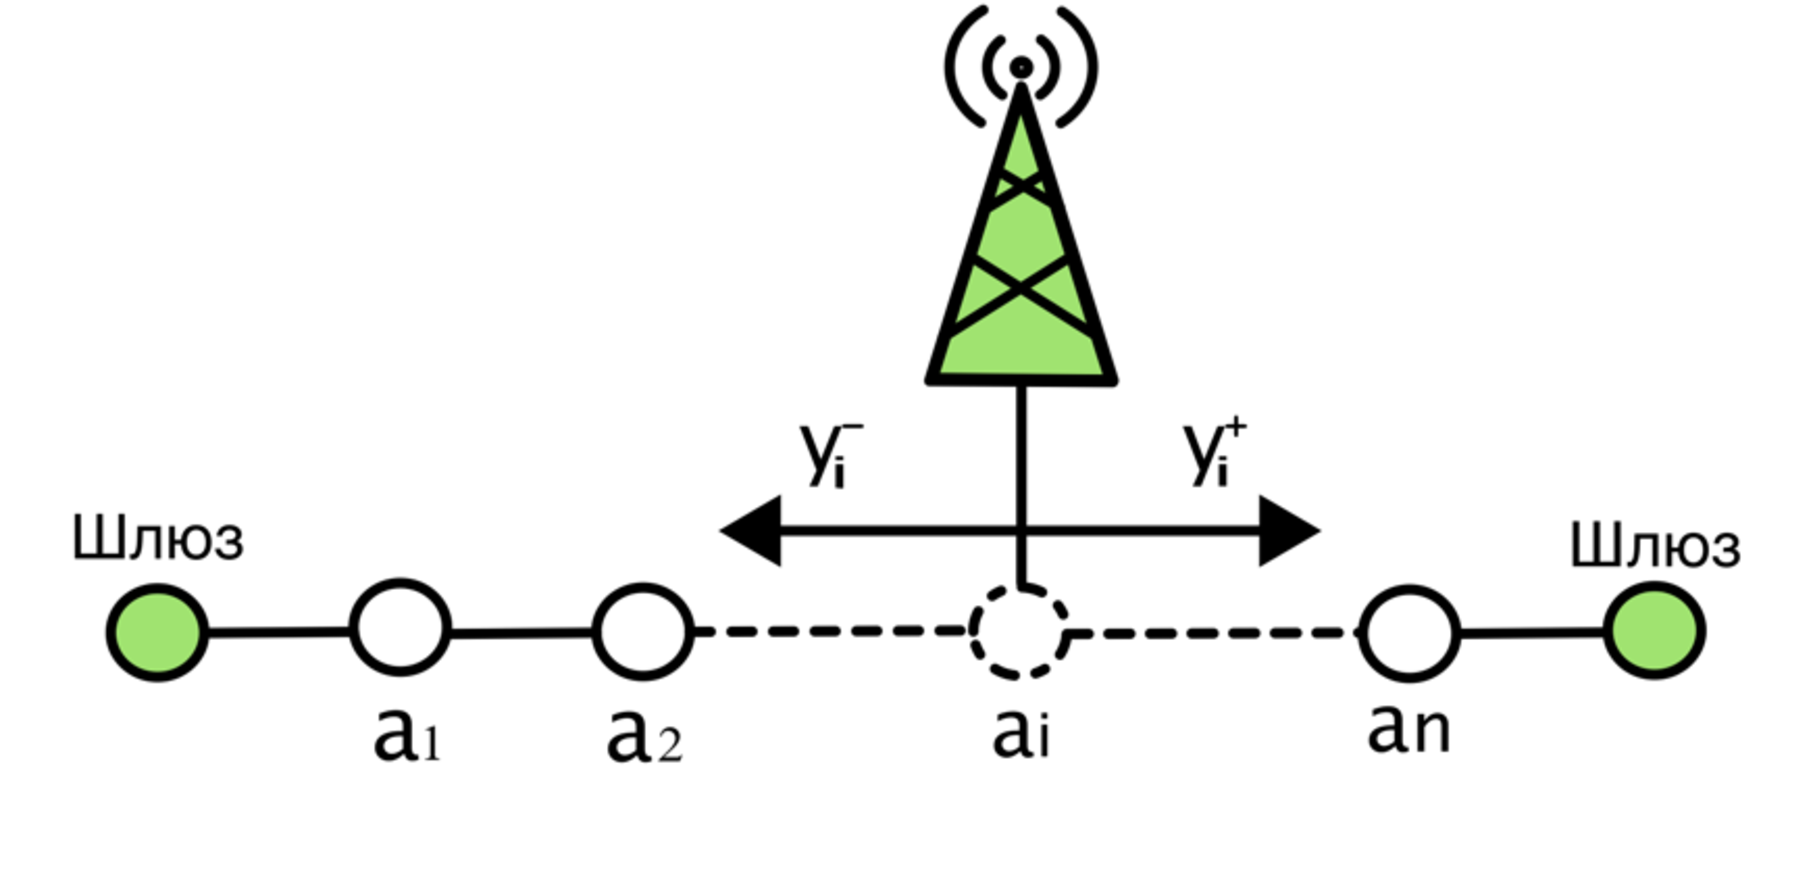
\includegraphics[scale=0.15]{station_coverage.pdf}}
        \center{\textbf{Охват покрытия станции}}
    \end{minipage}

    % \bigskip
    % \fontsize{8pt}{7.2}\selectfont
    % где $y_i^+$ и $y_i^-$ , $i= \overline{0,n+1}$ определяют охват покрытия (справа и слева, соответственно) станций.

\end{frame}

\begin{frame}
    \frametitle{задача ЦЛП}
    \begin{minipage}[t]{0.5\linewidth}
        \begin{equation}
            \label{eq:part3_ei}
            e_i =  \sum\limits_{j=1}^m x_{ij}, \quad i = \overline{1,n}. 
          \end{equation}
    \end{minipage}

    \begin{minipage}[t]{0.5\linewidth}
        % \fontsize{8pt}{7.2}\selectfont
        
    \bigskip
    \bigskip
    \bigskip
    Суммарное покрытие между двумя станциями не больше расстояния между ними.
          

    \end{minipage}
    \hfill
    \begin{minipage}[t]{0.47\linewidth}
        
        \center{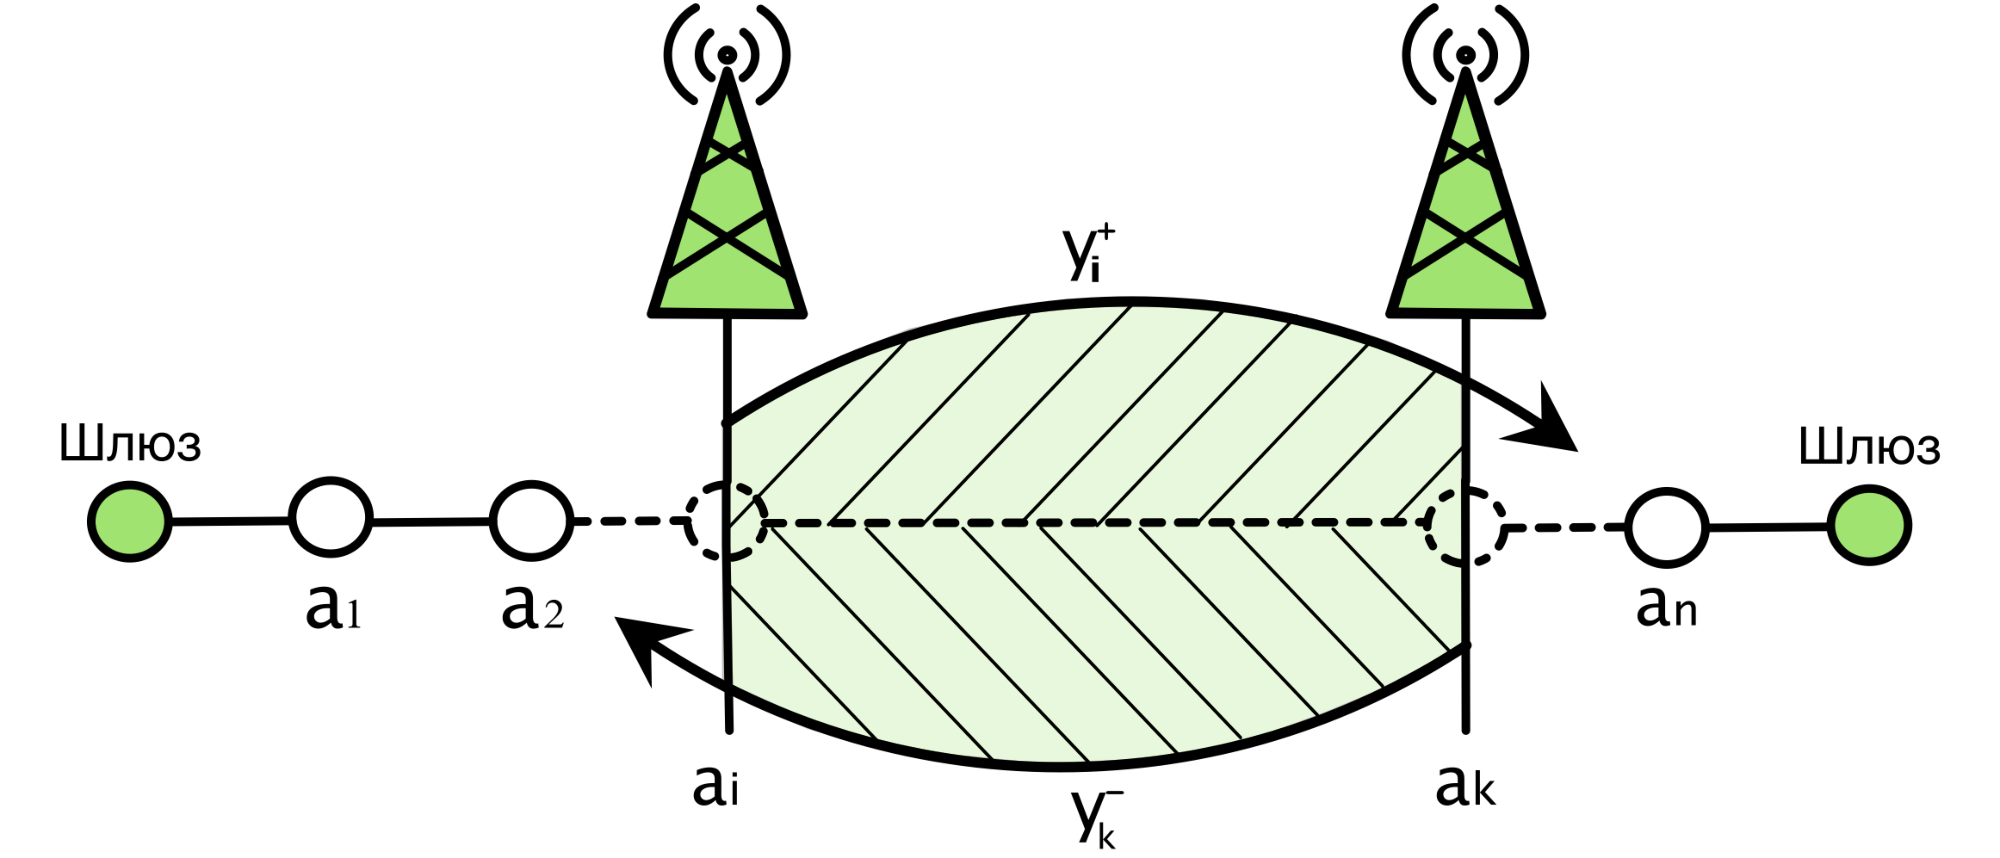
\includegraphics[scale=0.15]{total_coverage_between_points.pdf}}
        \center{\textbf{Покрытие между станциями}}
    \end{minipage}

    \bigskip
    \fontsize{8pt}{7.2}\selectfont
    \begin{equation}
        \label{eq:part3_yi_3}
        y_i^+ + y_k^- \leq \frac{l_k - l_i}{2} \cdot (e_i + e_k ) + (2 - e_i - e_k ) \cdot L, \quad i = \overline{1,n},  \quad k = \overline{i+1,n+1};
      \end{equation}
      
      \begin{equation}
        \label{eq:part3_yi_4}
        y_i^- + y_k^+  \leq \frac{l_i-l_k}{2} \cdot (e_i + e_k) + (2 - e_i - e_k) \cdot L, \quad i = \overline{1,n}, \quad k = \overline{i-1,0},
      \end{equation}

\end{frame}

\begin{frame}
    \frametitle{задача ЦЛП}
    \begin{minipage}[t]{1\linewidth}
        \fontsize{9pt}{7.2}\selectfont
        Введем переменные $z_{ijkq}, i = \overline{1,n}; j= \overline{1,m}; k=\overline{1,n},  k \neq i; q= \overline{1,m}, q \neq j$.
    \bigskip
    $$
    z_ {ijkq} = 
     \begin{cases}
       1& \text{, если в точке $ a_i $ размещена станция $ s_j $} \\
        & \text{и данная станция связана со станцией} \\
        & \text{$ s_q $, размещенная в точке $ a_k $;} \\
       0 & \text{, в противном случае.}
     \end{cases}
    $$
    \bigskip
    \end{minipage}
    
    \begin{minipage}[b]{0.5\linewidth}
        Важно обеспечить связь любой станции со шлюзами на концах участка через систему размещенных станций. 

    \end{minipage}
    \hfill
    \begin{minipage}[t]{0.47\linewidth}
        
        \center{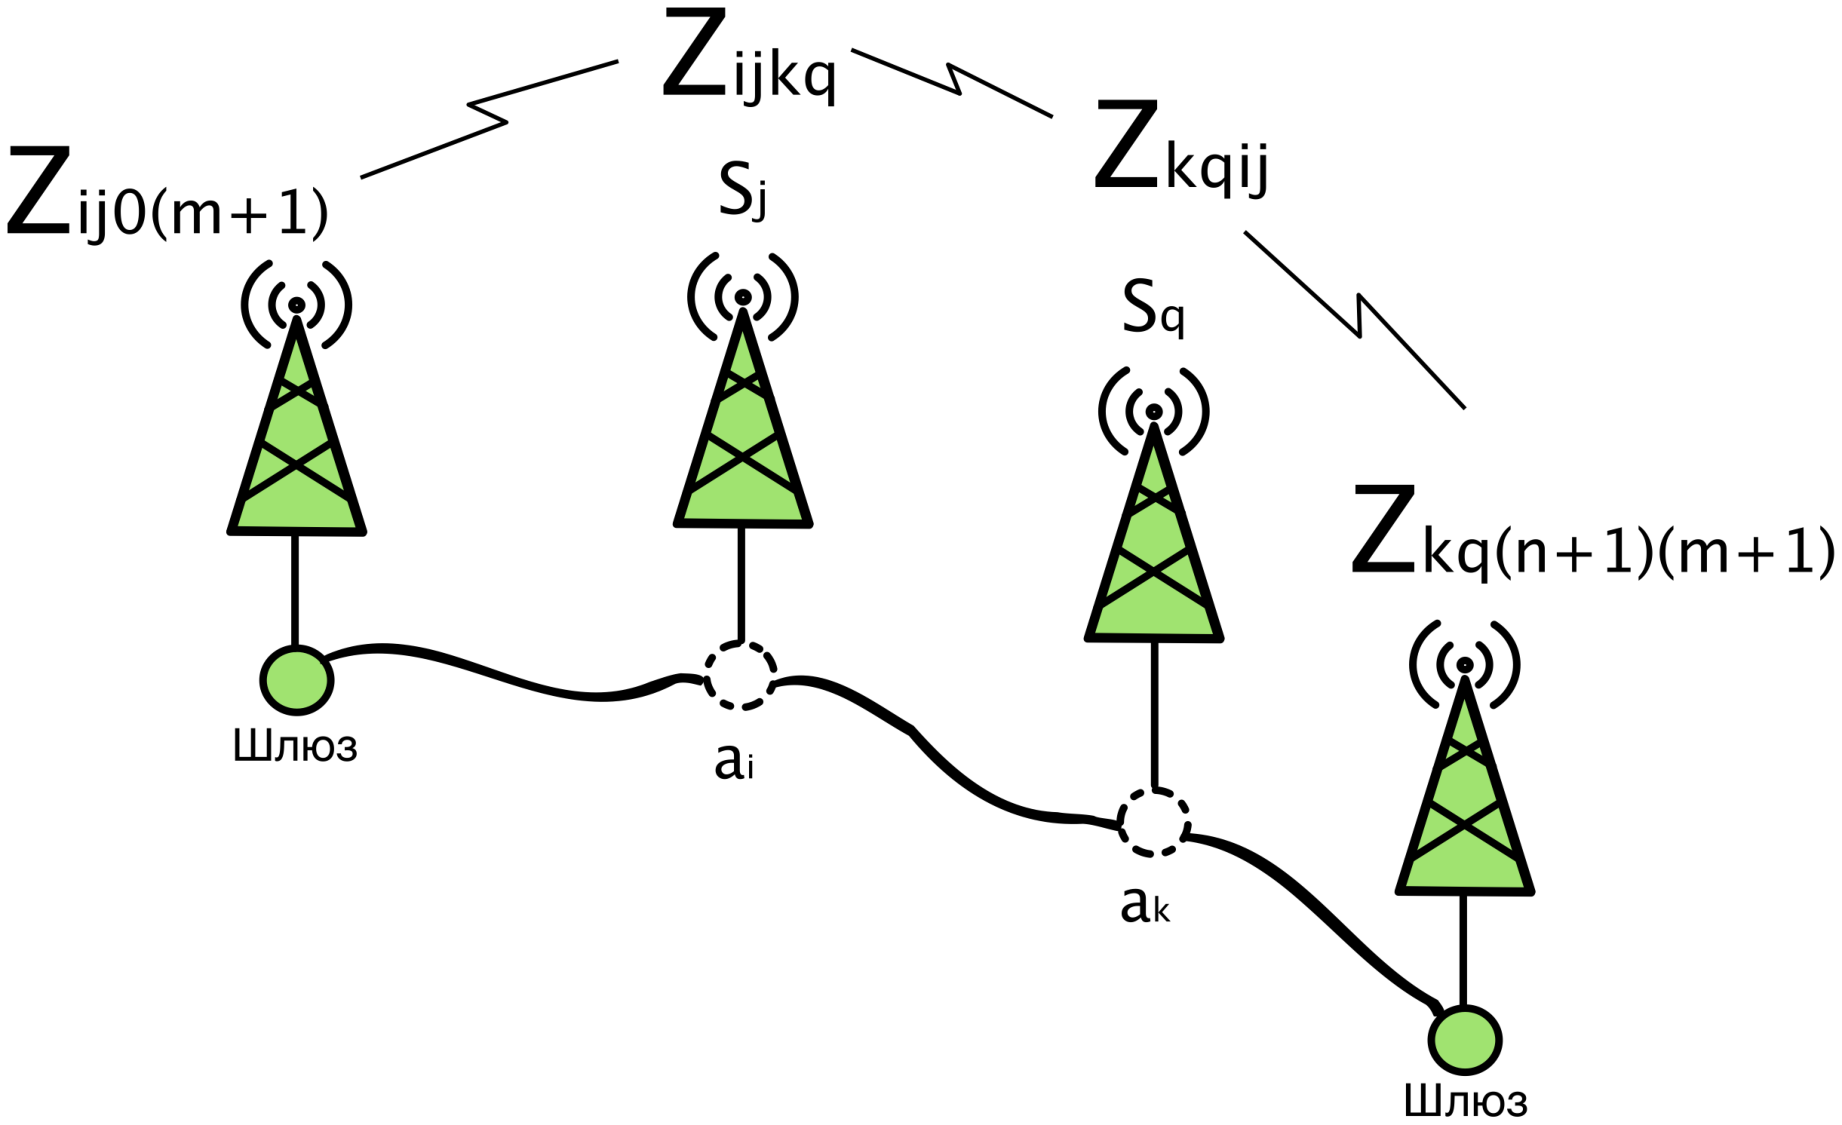
\includegraphics[scale=0.15]{station_link.pdf}}
        \center{\textbf{Связь между станциями}}
    \end{minipage}

\end{frame}


\begin{frame}[plain, noframenumbering]
    \frametitle{задача ЦЛП}
    
    \begin{minipage}[t]{0.99\linewidth}
        \fontsize{8 pt}{7.2}\selectfont
        \begin{equation}
            \label{eq:part3_z_ijkq_1}
            z_{ijkq} \leq e_i , \quad i = \overline{1, n}; \quad j = \overline{1, m}; \quad k = \overline{1,n}, k \neq i; \quad q = \overline{1,m}, q \neq j;
        \end{equation}
        
        
        \begin{equation}
            \label{eq:part3_z_ijkq_2}
            z_{ijkq} \leq e_k , \quad k = \overline{1, n}; \quad j = \overline{1, m}; \quad i = \overline{1,n}, i \neq k; \quad q = \overline{1,m}, q \neq j.
        \end{equation}
        
        
        \begin{equation}
            \label{eq:part3_z_ijkq_3_1}
            \sum\limits_{k=i+1}^{n} \sum\limits_{\substack{q = 1\\ q \neq j}}^m z_{ijkq} + z_{ij(n+1)(m+1)} = x_{ij} ,  \quad i = \overline{1, n}, \quad j = \overline{1, m}.
        \end{equation}

        
        \begin{equation}
            \label{eq:part3_z_ijkq_3_2}
            z_{nj(n+1)(m+1)} = x_{nj} \quad j = \overline{1, m}.
        \end{equation}

        
        \begin{equation}
            \label{eq:part3_z_ijkq_4_1}
            z_{1j0(m+1)}= x_{ij}, \quad j = \overline{1, m};
        \end{equation}

        
        \begin{equation}
            \label{eq:part3_z_ijkq_4_2}
            z_{ij0(m+1)} + \sum\limits_{k=1}^{i-1} \sum\limits_{\substack{q = 1\\ q \neq j}} z_{ijkq}= x_{ij}, \quad i = \overline{2, n}, \quad j = \overline{1, m}.
        \end{equation}

        
        \begin{equation}
            \label{eq:part3_z_ijkq_5}
            \sum\limits_{i=k+1}^{n} \sum\limits_{\substack{j=1 \\ j \neq q}}^m z_{ijkq} = x_{kq} , \quad k = \overline{1, n-1}, \quad q = \overline{1, m};
        \end{equation}

        
        \begin{equation}
            \label{eq:part3_z_ijkq_6}
            \sum\limits_{i=1}^{k} \sum\limits_{\substack{j=1 \\ j \neq q}}^m z_{ijkq} = x_{kq} , \quad k = \overline{2, n}, \quad q = \overline{1, m};
        \end{equation}
    \end{minipage}

\end{frame}


\begin{frame}
    \frametitle{задача ЦЛП}
    \begin{minipage}[t]{1\linewidth}
        \fontsize{6pt}{7.2}\selectfont
        $\forall i= \overline{1,n}$:
        \begin{equation}
          \label{eq:part3_z_ijkq_7}
          z_{ijkq}(R_{jq}-(a_i-a_k ))\geq 0, \quad k=\overline{0,i-1}; \quad j=\overline{1,m}; \quad q= \overline{1,m}, q \neq j; 
        \end{equation}
        
        \begin{equation}
          \label{eq:part3_z_ijkq_8}
          z_{ijkq} (R_{jq}-(a_k-a_i )) \geq 0, \quad k=\overline{i+1,n+1}; \quad j=\overline{1,m}; \quad q= \overline{1,m}, q \neq j.
        \end{equation}
    \bigskip
    \end{minipage}
    
    \begin{minipage}[и]{0.5\linewidth}
        \fontsize{8pt}{7.2}\selectfont
        Радиусы связи размещенных станций должнs быть не меньше расстояния между ними
        \bigskip
        \bigskip
        \bigskip

    \end{minipage}
    \hfill
    \begin{minipage}[b]{0.47\linewidth}
        
        \center{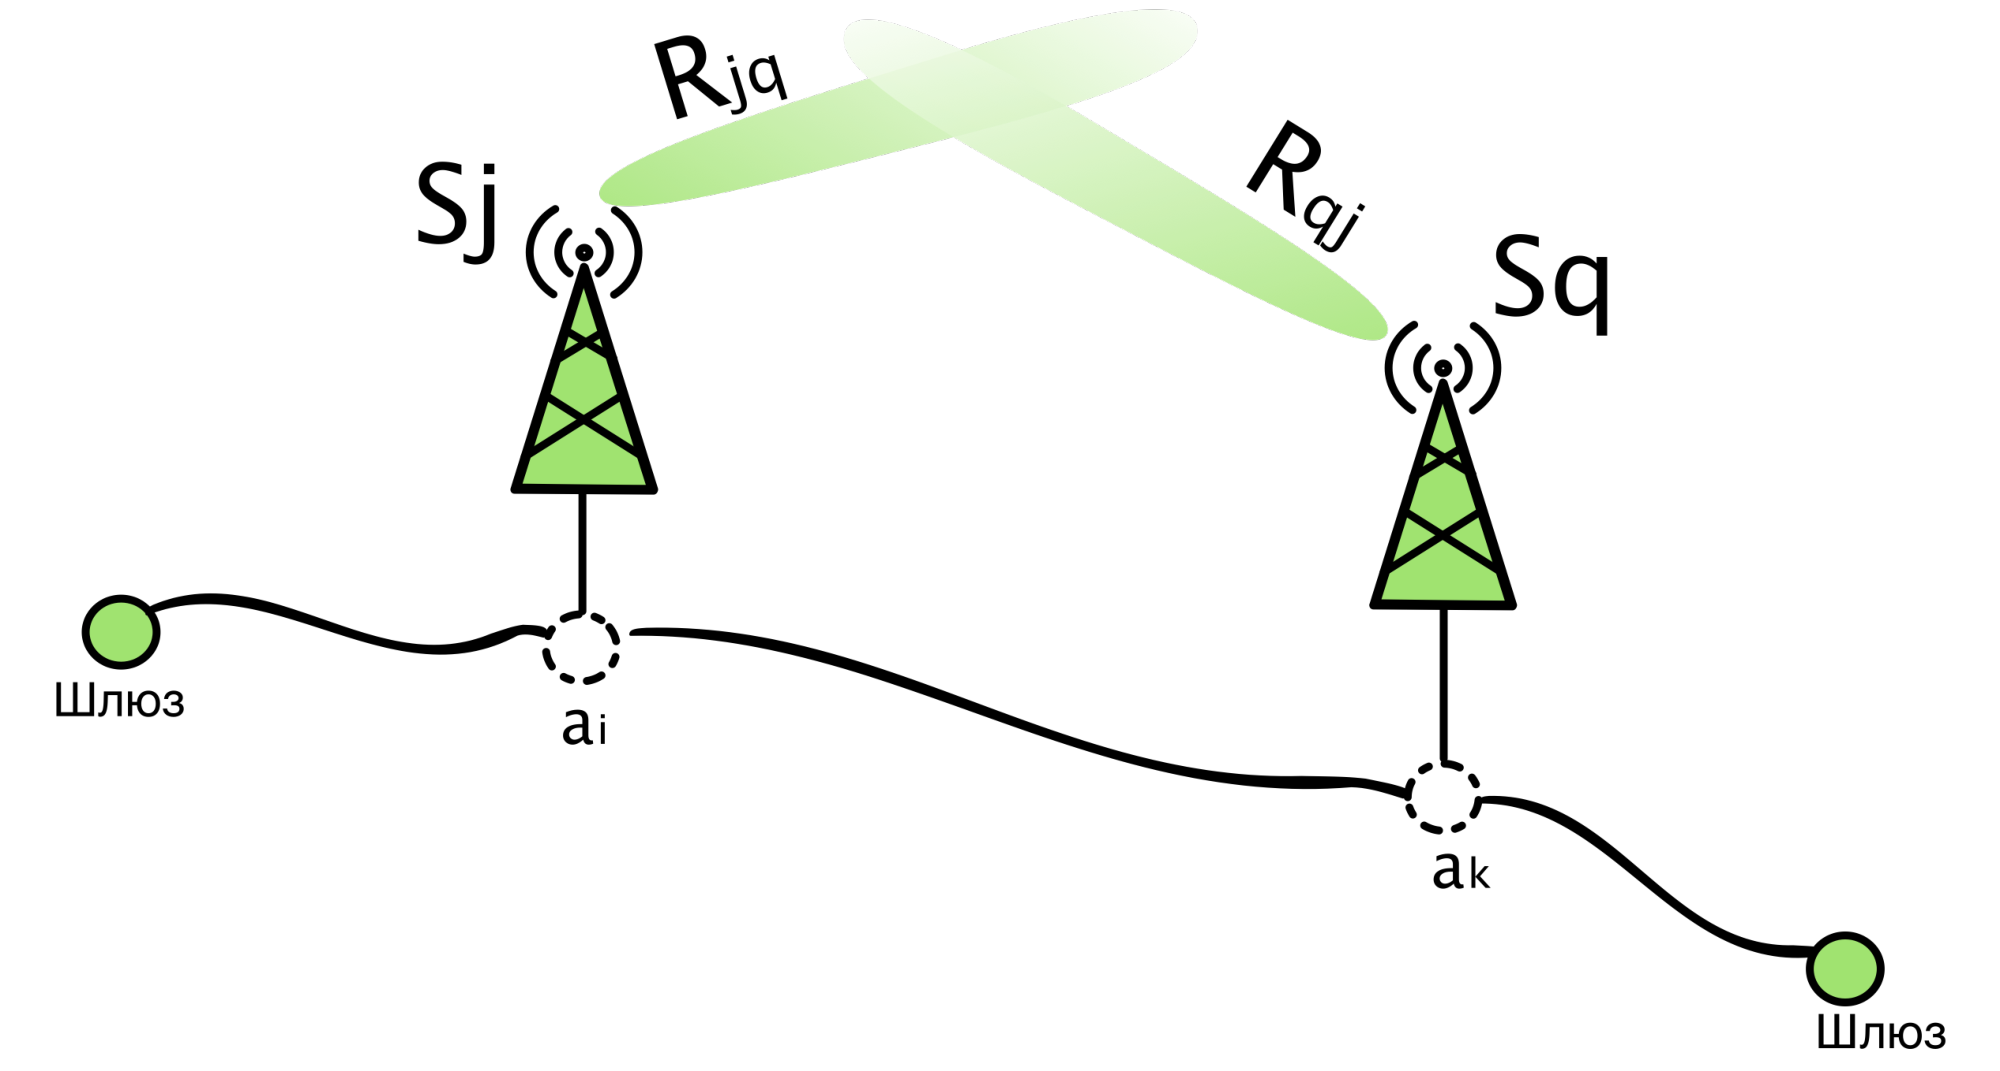
\includegraphics[scale=0.1]{station_link_between_points.pdf}}
        \center{\textbf{Обеспечение связи с соседней станцией}}
    \end{minipage}
    % \hfill
    \begin{minipage}[b]{0.99\linewidth}
        \fontsize{8pt}{7.2}\selectfont
        И бюджетное ограничение:

        \begin{equation}
        \label{eq:part3_cost}
        \sum\limits_{i=1}^n \sum\limits_{j=1}^m x_{ij} \cdot c_j \leq C.
        \end{equation}
    \end{minipage}

\end{frame}

\begin{frame}
    \frametitle{задача ЦЛП}
    \justifying
    
    Работа$^1$ содержит доказательство NP-полноты для частного случая задачи ЦЛП, когда вдоль линейной территории размещают множество однотипных станций с одинаковыми параметрами. 
    \bigskip
    
    Представленная в данном исследовании модель (1) - (18) рассматривает общий случай размещения, когда вдоль линейного участка размещают множество различных станций с разными техническими параметрами. Следовательно, данная задача является также NP-полной.
    \bigskip

    Представленная математическая модель рассчитывалась в пакете
    
    Optimization Toolbox MATLAB.
    % Представленная математическая модель рассчитывалась алгоритмом Лэнд и Дойг (1960).
    \bigskip

    \bigskip
    \bigskip
    \begin{minipage}[b]{0.99\linewidth}
        \fontsize{6pt}{7.2}\selectfont
    1. On a problem of base stations optimal placement in wirelessnetworks with linear topology. — [текст]. / — R. Ivanov [и др.] //Communications in Computer and Information Science. — 2018. —т. 919. — с. 505—513.
    \end{minipage}

\end{frame}

\begin{frame}
    \frametitle{Комбинаторная модель}
    \justifying

    \begin{itemize}
        \item ограничение на время межконцевой задержки сети невозможно привести к линейному виду;
        \item алгоритмы решения общего вида задач ЦЛП не учитывают специфику конкретной задачи.
    \end{itemize}
    

    \bigskip
    Разработан специальный алгоритм размещения базовых станций \textbf{метода ветвей и границ (МВиГ)} для комбинаторной модели в экстремальной форме.

    \bigskip
    \textit{Допустимой расстановкой станций} назовем такой возрастающий по величине координат $l_i$  набор пар $P = \{a_i, s_j\},a_i \in A,i \neq 0,i \neq n+1;s_j \in S$.
    % \end{minipage}

\end{frame}

\begin{frame}
    \frametitle{Комбинаторная модель}
    \justifying
    Для каждой расстановки выполняются требования:

    \begin{enumerate}
        \item  для каждой пары $(a_i,s_j)$:
            \begin{itemize}
                \item слева: либо найдется такая пара $(a_k,s_q)$, что, $l_i - l_k \leqslant R_{jq}$  и $l_i - l_k  \leqslant R_{qj}$, либо $l_i-l_0 \leqslant R_{j0}$ и $l_i - l_0 \leqslant R_{0j}$;
                \item справа: либо найдется такая пара $(a_t,s_g)$, что, $l_t-l_i \leqslant R_{jq}$ и $l_t - l_i \leqslant R_{qj}$, либо $l_{n+1}-l_i \leqslant R_{j(m+1)}$ и $l_{n+1}-l_i \leqslant R_{(m+1)j}$. 
            \end{itemize}
    Данное требование гарантирует, что любая станция может быть связана со станциями на концах отрезка либо через промежуточные станции, либо непосредственно;
        \item в одной точке стоит не более одной станции;
        \item сумма задержек по всем размещенным станциям меньше заданной величины $T$ – средней межконцевой задержки по времени по всей системе станций;
        % \begin{displaymath}
        %     \label{eq:part3_e2e_delay}
        %     \sum\limits_{j \in S_\sigma} \overline{T_j} \leqslant T,
        % \end{displaymath}
    % где $S_\sigma$ – множество размещенных станций, $\overline{T_j}$ -- среднее время задержки на станции.
        \item суммарная стоимость размещенных станций меньше заданного бюджетного ограничения  $C$.
    \end{enumerate}

\end{frame}

\begin{frame}
    \frametitle{Комбинаторная модель}
    \justifying
    Каждой допустимой расстановке станций $P$ соответствует величина покрытия $z(P)$, определяемая как суммарная область покрытия станции, входящих в набор пар $P$.

    Для удобства описании в дальнейшем алгоритмов введем понятие «недопокрытия»:

    \begin{displaymath}
        f(P) = L - z(P)
    \end{displaymath} 

    \textbf{Задача 1.}
    Пусть $G$ -- множество всех допустимых расстановок $P$.

    \bigskip

    Тогда требуется найти такую допустимую расстановку  $P^*$, что
    \begin{displaymath}
        \label{eq:present_P}
        P^* = \argmin \limits_{P \in G} f(P)
    \end{displaymath}
\end{frame}

\begin{frame}
    \frametitle{Комбинаторная модель}
    \justifying
    \begin{minipage}[t]{1\linewidth}
        \fontsize{8pt}{7.2}\selectfont
        \textbf{Процедура построения бинарного дерева поиска} 
        \bigskip

        На каждой итерации, начиная с итерации $\nu=0$, разбиваем текущее подмножество $G_\nu$ на два подмножества $G^1_\nu$ и $G^2_\nu$. 
    \bigskip
    \end{minipage}
    
    \begin{minipage}[b]{0.5\linewidth}
        \fontsize{8pt}{7.2}\selectfont
        В качестве параметра разбиения воспользуемся переменной $\pi_{ij}$:

        \begin{itemize}
            \item $\pi_{ij}=1$, если наложено условие, что на месте $a_i$ расположена станция $s_j$;
            \item $\pi_{ij} = 0$, если наложено условие, что на месте $a_i$ станция $s_j$  располагаться не будет.
        \end{itemize}
        \bigskip

    \end{minipage}
    \hfill
    \begin{minipage}[b]{0.47\linewidth}
        
        \center{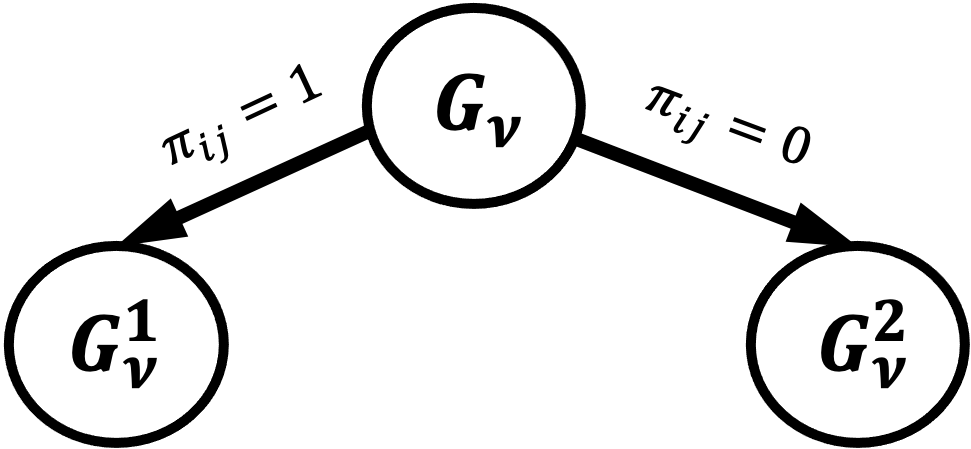
\includegraphics[scale=0.5]{binary_tree.png}}
        \center{\textbf{Узлы бинарного дерева поиска}}
    \end{minipage}
    \hfill
    \begin{minipage}[b]{1\linewidth}
        \fontsize{8pt}{7.2}\selectfont
        \textbf{Алгоритм метода ветвей и границ.}
        \bigskip

        Для построения алгоритма МВиГ были разработаны методы исследования вершин дерева на возможность их закрытия.
        \bigskip

        % В соответствии с техникой МВиГ закрытие вершины в результате исследования, соответствующего ей множества $G_\nu$ возможно \textbf{в трех случаях}:
    \end{minipage}

\end{frame}

% \begin{frame}
%     \frametitle{Комбинаторная модель}
%     \justifying
%     \underline{\textit{\textbf{Случай 1.}}} Множество $G_\nu$ -- пусто, т.е. доказано, что в множестве $G_\nu$ при данном наборе фиксированных и запрещенных переменных $\pi_{ij}$ нет ни одной допустимой расстановки $P$.
%     \bigskip

%     \underline{\textit{\textbf{Случай 2.}}} Доказано, что в множестве $G_\nu$ не может быть допустимой расстановки $P$ с меньшим значением целевой функции (19), чем у лучшей расстановки $\widehat{P}$ из уже найденных. 
%     \bigskip 
    
%     \underline{\textit{\textbf{Случай 3.}}} Найдено оптимальное решение на множестве $G_\nu$.
%     % Прежде чем рассмотреть эти три случая, запишем важное свойство любого множеств $G_\nu$, являющееся следствием принятого правила выбора свободной переменной для разбиения очередного множества $G_\nu$ при прямом шаге.

% \end{frame}

\begin{frame}
    \frametitle{Комбинаторная модель}
    \justifying
    На каждом узле проводится оценка "недопокрытия"  в виде суммы

    \begin{displaymath}
        W\left(G_\nu\right) = w_1\left(G_\nu \right) + w_2\left(G_\nu \right). 
    \end{displaymath}

    \begin{itemize}
        \item $w_1 \left(G_\nu \right)$ -- сумма все частичных «недопокрытий» слева от точки размещения и величины радиуса покрытия, размещаемой станций;
        \item $w_2 \left(G_\nu \right)$ вычисляется «для недопокрытия» справа на части $\beta$ до конца всего отрезка (точки $a_{n+1}$).
    \end{itemize}
    Оценку $w_2 \left(G_\nu \right)$ получим релаксацией условий, определяющих допустимую расстановку станций на участке $\beta$. Найдем такое подмножество $S_\beta$ множества станций $S$, состоящее из еще не размещенных станций и дающее минимальное «недопокрытие» на участке $\beta$ при выполнении только условий 2) – 4). 
    
\end{frame}

\begin{frame}
    
    \frametitle{Комбинаторная модель}
    \fontsize{8pt}{7.2}\selectfont
    Для этого сформулируем следующую задачу булевого программирования.

    \underline{\textit{\textbf{Задача 2.}}}
    \begin{displaymath}\label{present:task2}
        z = |\beta| - \sum\limits_{x_j \in S_\beta} r_j x_j \rightarrow min.
    \end{displaymath}

    \begin{displaymath}\label{eq:part4_task2_cost}
        \sum\limits_{x_j \in S_\beta} c_j x_j \leqslant C,
    \end{displaymath}

    \begin{displaymath}\label{eq:part4_task2_m}
        \sum\limits_{x_j \in S_\beta} x_j \leqslant m,
    \end{displaymath}

    \begin{displaymath}
        x_j \in \{0, 1\},
    \end{displaymath}
    где $|\beta|$ -- длина отрезка отрезка  $\beta$, $m$ -- число свободных мест для размещения станций на отрезке $\beta$.

    \bigskip
    Эффективность использования оценки в методе ветвей и границ определяется точностью оценки и временем ее вычисления. \underline{\textit{\textbf{Задача 2}}} -- это задача ЦЛП, являющаяся труднорешаемой. 

    При снятии любого одного из ограничений \underline{\textit{\textbf{задача 2}}} представляет собой целочисленную задачу о ранце c эффективным псевдополиномиальным алгоритмом решения.
    % На основании \underline{\textit{\textbf{задачи 2}}} можно получить две оценки менее точные, но имеющие более эффективные методы решения. 
    
    % Заметим, что при снятии любого одного из ограничений \underline{\textit{\textbf{задача 2}}} представляет собой целочисленную задачу о ранце c эффективным псевдополиномиальным алгоритмом решения. При этом с точки зрения точности оценки, более перспективным представляется снятие ограничения на число свободных мест $m$, так как на практике, обычно, число возможных мест размещения станций существенно меньше числа размещенных станций, полученного в результате решения задачи. 
    \bigskip
    Если множество $G_\nu$ получено из материнского добавлением условия $\pi_{ij}=0$, то оценка $W(G_\nu)$ равна оценке материнского множества.

\end{frame}

\begin{frame}
    \fontsize{8pt}{7.2}\selectfont
    \frametitle{Комбинаторная модель}
    \justifying
    Если для найденной расстановки $P$ выполняются условия 1) – 4), которые для единственной расстановки легко проверяются, и

    \begin{displaymath}
        f(P) < f(\widehat{P}),
    \end{displaymath}
    то $f(P)$ принимается за новый рекорд $f(\widehat{P})$, расстановка $P$ становиться новым рекордным решением $\widehat{P}$ и выполняется шаг обратного хода по дереву поиска. Если неравенство не выполняется, то рекорд остается прежним и выполняется шаг обратного хода.

    \bigskip
    Работа алгоритма МВиГ заканчивается, когда все вершины дерева поиска закрыты, при этом решение задачи: 

    \begin{displaymath}
        P^{*} = \widehat{P},  f(P^*) = f(\widehat{P}).
    \end{displaymath}

    \bigskip
    \bigskip
    % Обе задачи, в виде ЦЛП и в виде комбинаторной модели в экстремальной форме относятся к широкому к \textbf{классу задач размещения мощностей}. Отличительной особенностью рассмотренных задач является наличие условия на связь между размещаемыми объектами и линейная контролируемая территория.
\end{frame}

\begin{frame}
    \frametitle{Численный результат}

    Требуется разместить весь набор $m$ имеющихся однотипных станций. Множество всех возможных вариантов комбинаций $m$ станций на  $n$ местах запишем как $\Gamma$. Общее количество $\gamma \in \Gamma$:
    В МВиГ отпустим ограничение на межконцевую задержку.
    \begin{displaymath}
    \gamma = C_n^m \times m!.
    \end{displaymath} 
 
    Характеристика сравенения двух моделей --  \textbf{количество пройденных узлов} в ходе поиска оптимального значения.

    % В таблице показаны результаты решения задач для различного числа количества размещения и количества станций с использованием полного перебора, алгоритма МВиГ и модели ЦЛП. Для каждого набора станций и набора размещений были рассчитаны 10 примеров с различными числовыми входными данными. Для <<$-$>> решение задачи данной размерности методом полного перебора не было получено за 3 ч счета. 

    % Как видно из результов, представленных в таблице, при увеличении размерностей задачи, алгоритм МВиГ позволяет найти решение быстрее в ходе движения по дереву поиска.

    \begin{table}[b]\centering
        \caption{Результаты численного решения.}\label{tab:problems_BF_BnB_ILP}
        \begin{tabular}{|l|l|l|l|l|}
        \hline
        \textbf{Места} & \textbf{Станции} &	\textbf{Полный}& \textbf{МВиГ} & \textbf{ЦЛП} \\ 
        \textbf{размещения} &  &	\textbf{перебор}&  &  \\
        \hline
        7 &		5 &	17550  &	933 &		\textbf{753}\\
        9 &		5 &	71090  &	6478 &		\textbf{2669}\\
        10 &	5 &	126180 &	\textbf{1041} &		8551\\
        12 &	6 &	-- &		\textbf{8294} &		38569\\
        13 & 	6 &	-- &		\textbf{18485} &	30369\\
        \hline
        \end{tabular}
    \end{table}

\end{frame}

\begin{frame}
    \frametitle{Последовательность лучших решений}
    \fontsize{8pt}{7.2}\selectfont
    Рассмотрим \textbf{задачу 1.}

    \begin{displaymath}
        f(P^*) = min \{f(P), P \in G \}.
    \end{displaymath}

    Построим для этой задачи последовательность $\Gamma = P^1, P^2, ... ,P^k$ допустимых расстановок (решений) множества $G$ для заданного $k$, где 
    \begin{align}
        f(P^1) &= f(P^*), \nonumber  \\
        f(P^2) &= extr\{ f(P), P \in G \ P^1 \}, \nonumber \\
        ... \nonumber \\
        f(P^k) &= extr\{ f(P), P \in G \ P^1 \cup P^2 \cup ... P^k \}, \nonumber 
    \end{align} 
    
    Для итерационной процедура нахождения последовательности лучших решений достаточно неравенство $f(P) < f(\widehat{P})$ в алгоритме МВиГ заменить следующим неравенством 

    \begin{align}
        \label{eq:part4_is_less_than_record_d}
        f(P) \leqslant f(\widehat{P}) + d,
    \end{align}
    где $d = \varepsilon \cdot L > 0, \varepsilon$ -- заданное отклонение в процентах, и запоминать все рекорды, полученные в процессе решения задачи.

    % Увеличивая величину $d$, если при данном ее значении допустимого решения на этапе моделирования не найдено.
\end{frame}

\begin{frame}
    \frametitle{Выводы по Положениям 1, 2 и 3}
    \fontsize{8pt}{7.2}\selectfont

    \textbf{Представлены:}
    \begin{itemize}
        \item математическая модель ЦЛП;
        \item комбинаторная модель в экстремальной форме;
        \item специальный алгоритм МВиГ для комбинаторной модели;
        \item итерационная процедура нахождения последовательности лучших решений.
    \end{itemize}

    \bigskip
    \textbf{Публикации:}
    \begin{minipage}[c]{1\linewidth}
        \fontsize{6pt}{7.2}\selectfont
        \begin{enumerate}
            \item \textit{Иванов,Р. Е.Задача оптимального размещения заданного множе­ства базовых станций беспроводной сети связи с линейной топо­логией [Текст] / Р. Е. Иванов, А. А. Мухтаров, О. Першин //Автоматизация, телемеханизация и связь в нефтяной промышлен­ности. — 2019. — Т. 549, No 4. — С. 39—45};
            
            \item \textit{Ivanov,R.A Problem of Optimal Location of Given Set of Base Sta­tions in Wireless Networks with Linear Topology[Текст]/ R. Ivanov,A. Mukhtarov, O. Pershin // Communications in Computer and Infor­mation Science. –– 2019. –– Vol. 1141 CCIS. –– P. 53––64. –– (Scopus,WoS)};
            
            \item \textit{Мухтаров,А. А.Математические  модели  задачи  размещениябазовых станций для контроля линейной территории [Текст] /А. А. Мухтаров, Р. Е. Иванов, О. Ю. Першин // Proceedings of the22nd International Scientific Conference on Distributed Computer andCommunication Networks: Control, Computation, Communications(DCCN-2019, Moscow). — 2019. — С. 205—212};
            
            \item \textit{On Optimal Placement of Base Stations in Wireless Broadband Net­works to Control a Linear Section with End-to-End Delay Limited[Текст]/ A. Mukhtarov [et al.] // Communications in Computer andInformation Science. –– 2020. –– Vol. 1337. –– P. 30––42};
            
            \item \textit{{Вишневский,В. М.Задача оптимального размещения базовыхстанций широкополосной сети для контроля линейной территориипри ограничении на величину межконцевой задержки [Текст] /В. М. Вишневский, А. А. Мухтаров, О. Першин // Материалы23-й Международной научной конференции "Распределенные ком­пьютерные и телекоммуникационные сети: управление, вычисление,связь"(DCCN-2020, Москва). — 2020. — С. 148—155}}.
        \end{enumerate}
    \end{minipage}

\end{frame}

% \section{Положение 4}
\begin{frame}
    \begin{center}
        {Положение 4 - математические модели для задач проектирования БШС с ячеистой
        топологией;}
    \end{center}
\end{frame}



\begin{frame}
    \frametitle{Постановка задачи}
    \fontsize{8pt}{7.2}\selectfont
    \justifying
    Задано множество вершин $A = a_i$, $i=\overline{0,n}$. Каждая вершина $a_i$ имеет координаты $\left\{ x_i, y_i \right\}$.
    
    \begin{minipage}[c]{0.47\linewidth}
        \fontsize{8pt}{7.2}\selectfont
        \bigskip

        Множество $A$ состоит из двух подмножеств: 
        \begin{itemize}
        \item $A_1$ -- множество вершин, с которых необходимо собирать информацию. Каждой вершине $a_i$ приписана   величина $v_i$ -- максимальный объем информации, снимаемой с объекта, расположенного на этой вершине;
        \item $A_2$ -- множество возможных мест размещения базовых станций. 
        \end{itemize}

        По определению

        $$
        A_1 \cup A_2 = \varnothing;
        $$

        $$
        A_1 \cap A_2 = A.
        $$

        
    \end{minipage}
    % \hfill
    % \vrule{}
    % \hfill
    \begin{minipage}[c]{0.47\linewidth}
        \center{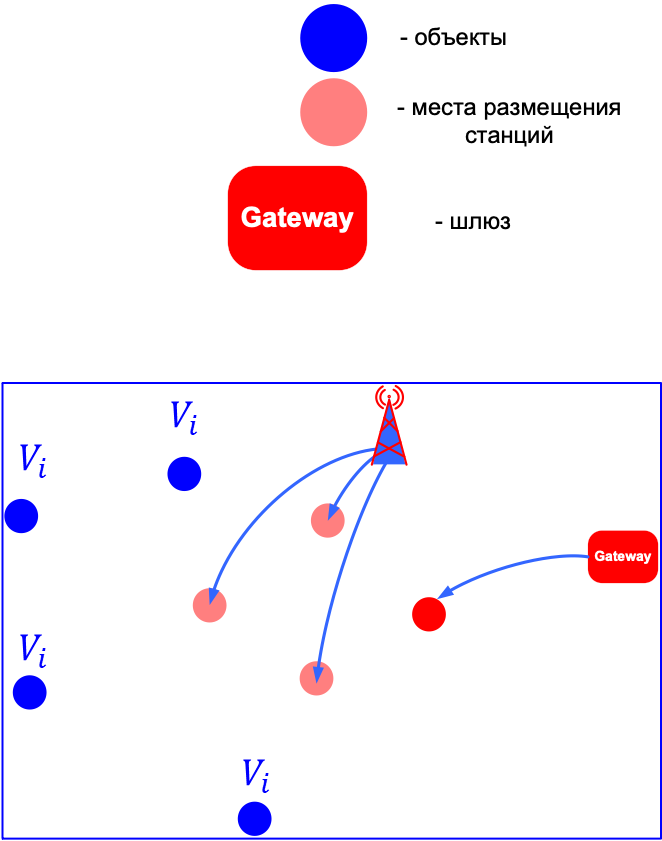
\includegraphics[scale=0.3]{A1A2.png}}
        \center{\textbf{Вершины $A$.}}
    \end{minipage}
    
    \bigskip
    \bigskip

    $
    A_1 = \left\{a_i \right\}, i= \overline{1,n_1};
    $ и $
    A_2 = \left\{ a_i  \right\}, i= \overline{n_1+1,n}.
    $
    
\end{frame}

\begin{frame}
    \frametitle{Постановка задачи}
    \justifying
    Задано множество типов базовых станций $S = s_j$, $j=\overline{1,m}$. Каждой станции приписаны параметры $s_j = \left\{r_j, R_{ij}, \vartheta_j, c_j \right\}$, где:
    $r_j$ -- максимальный радиус покрытия; $R_{ij}$ -- максимальный радиус связи между $i$-ой и $j$-ой станциями; $\vartheta_j$ -- максимальный объем информации в единицу времени, который может быть получен от объектов, обслуживаемых данной станцией; $c_j$ -- стоимость станции.
    
    \bigskip
    Требуется разместить станции таким образом, чтобы вся информация с объектов ($A_1$) могла быть собрана и передана системой станций до шлюза.

    \bigskip
    Задано условие, что информация c вершин множества $A_1$ может передаваться непосредственно только на вершины множества $A_2$, а со шлюзом и между собой могут быть связаны только вершины множества $A_2$.

\end{frame}


\begin{frame}
    \frametitle{Постановка задачи}
    \fontsize{8pt}{7.2}\selectfont
    Вместо каждой вершины множества $A_2$ введем $m$ вершин с координатами вершины $a_i$, и различными параметрами станций (множества $D_i$). Полученное множество по всем вершинам назовем $A_2D$.
    \bigskip

    Составим граф $H=\left\{AD,E\right\}$, передачи потока информации между вершинами расширенного множествa $AD=A_1 \cup A_2D$ и шлюзом.
    \bigskip

    Матрица смежности $E = \{e_{ij}\}$ графа $H$ строится по следующим правилам.
    
    \begin{minipage}[c]{0.47\linewidth}
        \fontsize{8pt}{7.2}\selectfont
        $$
        e_{ij} = 
        \begin{cases}
        1& \text{, если $ ||a_i - a_j|| \leqslant r_j, \forall i \in A_1, j \in A_2D$;} \\
        1 & \text{, если $ ||a_i - a_j|| \leqslant R_{ij}, \forall i \in A_2, j \in A_2D$;} \\
        1 & \text{, если $ ||a_i - a_0|| \leqslant R_{i0}, \forall j \in A_2D$;} \\
        0 & \text{, во всех остальных случаях.}
        \end{cases}
        $$
        \bigskip
        \bigskip
        \bigskip
        \bigskip
        \bigskip
        \bigskip
        
    \end{minipage}
    % \hfill
    % \vrule{}
    % \hfill
    \begin{minipage}[c]{0.45\linewidth}
        \bigskip
        \bigskip
        \bigskip
        \bigskip
        \bigskip
        \bigskip
        \center{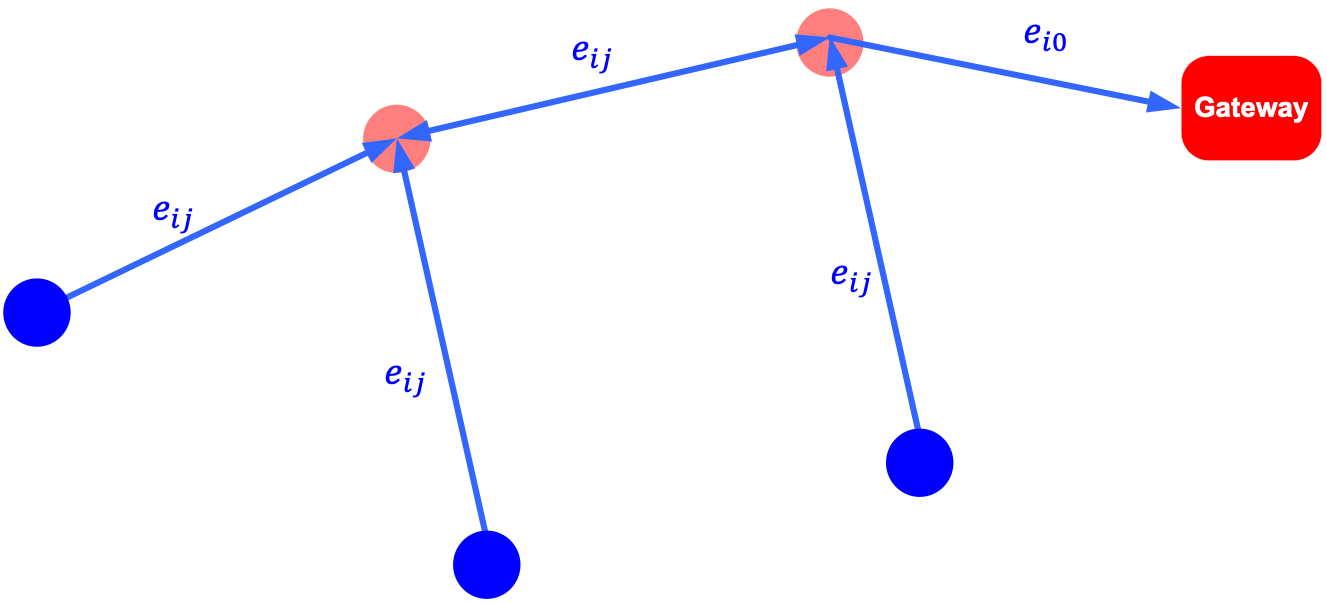
\includegraphics[scale=0.25]{adj_matrix.png}}
        \center{\textbf{Смежные вершины множества $A$}}
    \end{minipage}
    
\end{frame}


\begin{frame}
    \frametitle{Модель нахождение допустимого решения }
    \fontsize{8pt}{7.2}\selectfont
    \justifying
    Введем потоковые переменные $x_{ij} \geqslant 0$.

    \textbf{Величина суммарного потока с объектов через систему станций должна поступить на шлюз.}

    \begin{equation}\label{eq:part2_1.5}
        \sum_{a_j \in \Gamma^+(a_i)} x_{ij} = \vartheta_i, \forall a_i, i =\overline{1, n_1},
    \end{equation}
    \begin{minipage}[c]{1\linewidth}
        \fontsize{6pt}{7.2}\selectfont 
        где $\Gamma^+(a_i)$ -- множество вершин на графе $H$, в которые входят дуги, исходящие из вершины $a_i$.
    \end{minipage}

    \begin{equation}\label{eq:part2_1.6}
        \sum_{a_j \in \Gamma_1^-(a_i)} x_{ij} + \sum_{a_j \in \Gamma_2^-(a_i)} x_{ji} -  \sum_{a_j \in \Gamma_2^+(a_i)} x_{ij} =0 ,\forall a_i \in A_2, 
    \end{equation}

    \begin{minipage}[c]{1\linewidth}
        \fontsize{6pt}{7.2}\selectfont 
        где $\Gamma_1^-(a_i)$ -- вершины множества $A_1$, из которые выходят дуги, входящие в вершину $a_i$, $\Gamma_2^-(a_i)$ -- вершины множества $A_2D$, из которых выходят дуги, входящие в  вершину $a_i$, $\Gamma_2^+(a_i)$ -- вершины множества $A_2D$, в которые входят дуги, исходящие из вершины  $a_i$.
    \end{minipage}
    
    \begin{equation}\label{eq:part2_1.7}
        \sum_{a_j \in \Gamma_2^-(a_0)} x_{j0} = \sum_{a_i \in A_1} \vartheta_i,
    \end{equation}
    \begin{minipage}[c]{1\linewidth}
        \fontsize{6pt}{7.2}\selectfont 
        где $\Gamma_2^-(a_0)$ –- подмножество вершин множества $A_2D$, дуги которых входят в шлюз $a_0$.
    \end{minipage}

    \begin{equation}\label{eq:part2_1.8_1}
        \sum_{a_j \in \Gamma^-(a_i)} x_{ji} \leqslant  \vartheta_i, \forall a_i \in A_2D.
    \end{equation}

    \textbf{Задача (20) - (23) является задачей линейного программирования (ЛП) с функцией невязок уравнений ограничений в качестве целевой функции.}
    

\end{frame}

\begin{frame}
    \frametitle{Модель нахождение оптимального решения }
    \fontsize{8pt}{7.2}\selectfont
    % \justifying
    

    \begin{minipage}[c]{0.5\linewidth}
        Введем булевы переменные $y_i$ для вершин $a_i$, $a_i \in A_2D$:
    \begin{itemize}
        \item $y_i = 1$, если станция стоит на месте $a_i$;
        \item $y_i = 0$, в противном случае.
    \end{itemize}
        Заменим уравнение (23) на 
        \begin{equation}\label{eq:part2_1.8_2}
            \sum_{a_j \in \Gamma^-(a_i)} x_{ji} \leqslant y_i \cdot \vartheta_i, \forall a_i \in A_2D.
        \end{equation} 

        \begin{equation}\label{eq:part2_1.9}
            \sum_{a_j \in D_i} y_j \leqslant 1, \forall D_i.
        \end{equation}

        Целевая функция

        \begin{equation}\label{eq:part2_1.10}
            \sum_{a_i \in A_2D} c_i \cdot y_i \to min.
        \end{equation}
        \bigskip
        \bigskip

    \end{minipage}
    \hfill
    \begin{minipage}[c]{0.47\linewidth}
        \flushright
        \center{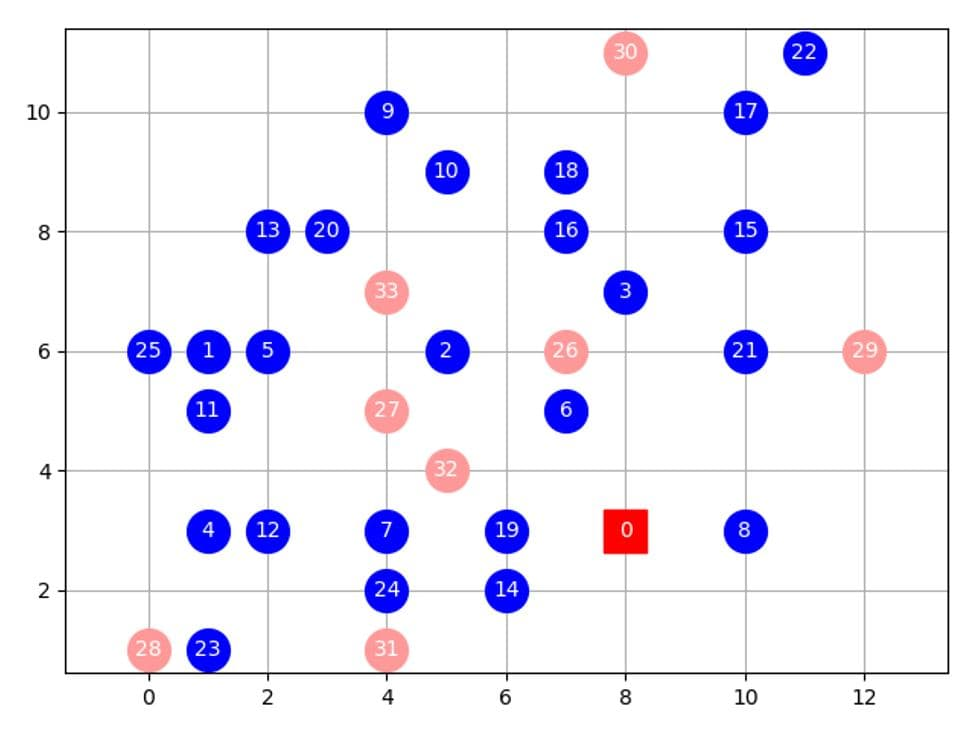
\includegraphics[scale=0.1]{input_A.png}}
        \center{\textbf{Множества заданных вершин}}
        \center{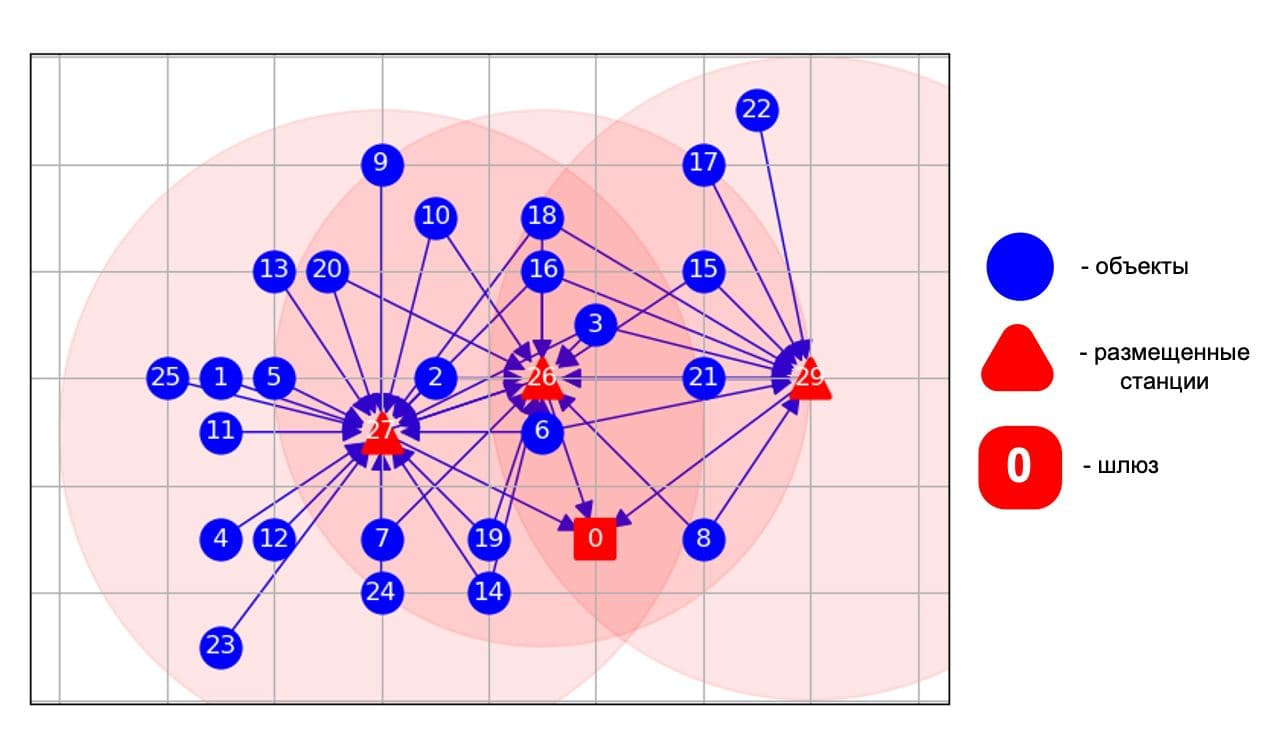
\includegraphics[scale=0.1]{output_A.png}}
        \center{\textbf{Оптимальное решение}}
    \end{minipage}

    Задача (20) - (22), (24) - 26) представляет собой частично целочисленную задачу линейного программирования (ЧЦЛП) с $m \cdot |A_2|$ булевыми переменными.
    
\end{frame}

\begin{frame}
    \frametitle{Выводы по Положению 4}
    \fontsize{8pt}{7.2}\selectfont

    В рамках широкого к \textbf{класса задач размещения мощностей} в наших задачах размещения есть специфика на связь между всеми узлами сети и в  наличие линейной траектории в случае задачи с линейной топологией. 
    \bigskip

    \textbf{Представлены:}
    \begin{itemize}
        \item математическая модель ЛП для проверки условия допустимого распределения по каналам связи;
        \item математическая модель ЧЦЛП оптимального размещения станций для контроля множества рассредоточенных объектов.
    \end{itemize}

    \bigskip
    \textbf{Публикации:}
    \begin{minipage}[c]{1\linewidth}
        \fontsize{6pt}{7.2}\selectfont
        \begin{enumerate}
            \item \textit{Мухтаров,А. А.Задача размещения базовых станций широкопо­лосной связи для обслуживания заданного множества рассредото­ченных объектов [текст] / А. А. Мухтаров, О. Ю. Першин // Труды 13-го Всероссийского совещания по проблемам управления (ВСПУXIII, Москва, 2019). — 2019. — с. 2992—2994.};
            
            \item \textit{Мухтаров,А. А.Оптимальное размещение базовых станций широ­кополосной беспроводной сети связи для обслуживания заданногомножества рассредоточенных объектов [текст] / А. А. Мухта­ров, О. Ю. Першин // Труды 12-й Международной конференции«Управление развитием крупномасштабных систем» (MLSD’2019,Москва). — 2019. — с. 531—537};
            
            \item \textit{Мухтаров,А. А.Оптимальное размещение базовых станций широ­кополосной беспроводной сети связи для обслуживания заданногомножества рассредоточенных объектов [текст] / А. А. Мухтаров,О. Ю. Першин // Материалы 12-й Международной конференции«Управление развитием крупномасштабных систем» (MLSD’2019,Москва). — 2019. — с. 610—612.};
            
        \end{enumerate}
    \end{minipage}

\end{frame}


% \section{Положение 5}
% \begin{frame}
%     \begin{center}
%         {Положение 5 - модели прогнозирования оценок характеристик производительности сети с
%         помощью методов машинного обучения для многофазной сети массового обслуживания с
%         зависимым временем обслуживания.}
%     \end{center}
% \end{frame}

% \begin{frame}
%     \justifying
%     \frametitle{Многофазная сеть массового обслуживания}
%     \fontsize{8pt}{7.2}\selectfont

%     Одним из важных ограничений для алгоритма МВиГ является межконцевая задержка сети $T$.
%     \bigskip

%     Для оценки данной характеристики используют стохастические модели массового обслуживания.
%     \center{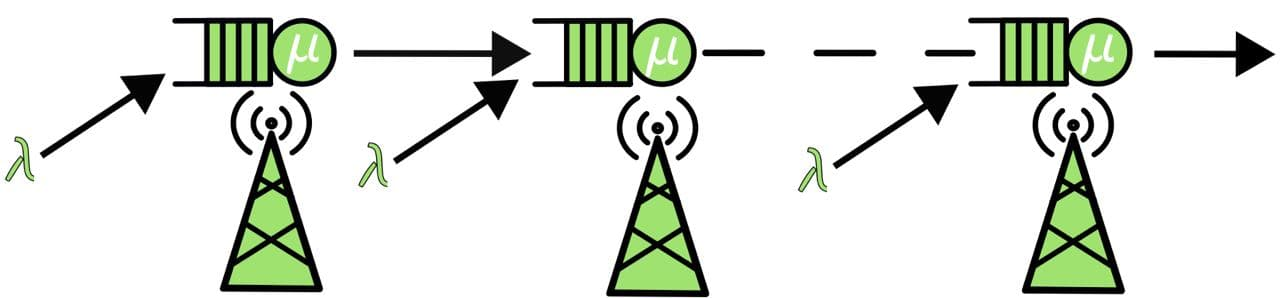
\includegraphics[scale=0.3]{tandem_queue.png}}
%     \center{\textbf{Многофазная сеть массового обслуживания}}

%     \bigskip

%     {В класическом случае для расчета межконцевой задержки сети рассматривают простейшую модель многафазной сети массового обслуживания  с узлами $M/M/1$ c линейной топологией и $N$ последовательно соединенными узлами. В такой системе  интервалы между поступлениями пакетов задается случайной величиной $A \sim Exp(\lambda)$ и время обслуживания с помощью случайной величины $S \sim Exp(\mu)$.}

   
% \end{frame}


\begin{frame}
    \justifying
    \frametitle{Оценка времени межконцевой задержки сети}
    \fontsize{8pt}{7.2}\selectfont

    % Для аналитического расчета межконцевой задержки сети $T$ предполагается допущение о \textbf{независимости длительности обслуживания на каждой фазе сети}.
    % \bigskip

    Для оценки данной характеристики используют стохастические модели сетей массового обслуживания.
    \center{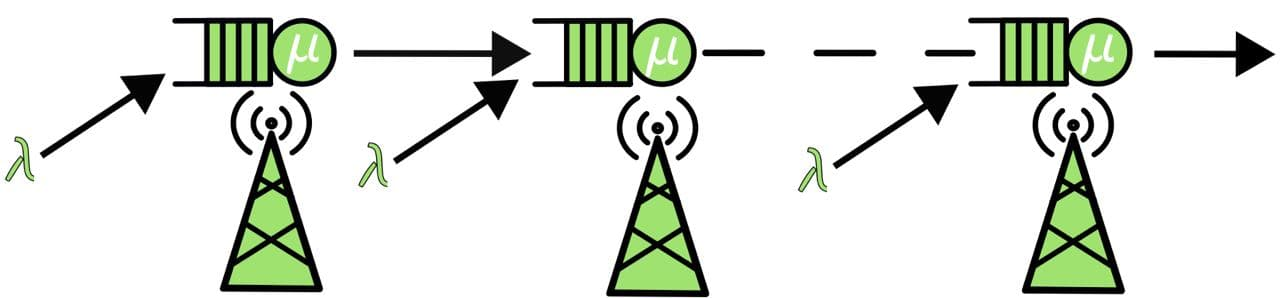
\includegraphics[scale=0.3]{tandem_queue.png}}
    \center{\textbf{Многофазная сеть массового обслуживания}}

    \bigskip

    Для сетей массового обслуживания (СеМО) с конечным буфером получить аналитическое решение для всей сети достаточно тяжело.

    \bigskip

    Одним из путей решений является использования имитационного моделирования многофазной сети.

\end{frame}

\begin{frame}
    \justifying
    \frametitle{Оценка времени межконцевой задержки сети}
    \fontsize{8pt}{7.2}\selectfont

    \textbf{Имитационное моделирование СеМО} представляет из себя метод Монте-Карло, в котором генерируют и прогоняют несколько сотен тысяч пакетов для оценки характеристик производительности сети.

    \bigskip

    \textbf{Недостаток} -- большие трудозатраты по времени.
    \bigskip

    \textbf{Решение} -- для задачи поиска оптимального размещения аппроксимировать данные имитационного моделирования с помощью методов машинного обучения. 
    \bigskip

    На вход имитационной модели подавались:
    \begin{itemize}
        \item $N$ -- число станций в сети;
        \item $M$ -- размер буфера очередей на фазах;
        \item $m_A$ -- cреднее значение случайного времени между поступлениями пакетов;
        \item $\sigma_A$ -- стандартное отклонение случайного времени между поступлениями пакетов;
        \item $R$ -- битовая скорость;
        \item $m_C$ -- cреднее значение случайного размера пакетов;
        \item $\sigma_C$ -- стандартное отклонение случайного пакетов;
    \end{itemize}
    \bigskip

    По среднии значениям и стандартным отклонениям проводилась апроксимация функций распределений. Если коэффициент вариации $c_v = \frac{\sigma}{m} < 1$, то распределение принадлежит распределения Эрланга. Если $c_v =1$, то экспоненциальному закону. Если $c_v > 1$, то случайная величина принадлежит гиперэкспоненциальному распределению. 

    На выходе рассчитывалась межконцевая задержка сети $\overline{T}$. 

\end{frame}

\begin{frame}
    \justifying
    \frametitle{Оценка времени межконцевой задержки сети}
    \fontsize{8pt}{7.2}\selectfont

    Было сгенирована выборка объемом 80000 строчек. Методом Монте-Карло для каждого случая прогонялось 100000 пакетов. 
    \bigskip
    
    \begin{minipage}[c]{0.47\linewidth}
        

    Регрессионные модели строились с помощью
    \begin{itemize}
        \item МНК;
        \item дерева принятия решения;
        \item градиентного бустинга;
        \item искусственные нейронные сети на алгоритме Адам.
    \end{itemize}

    \end{minipage}
    \hfill
    \begin{minipage}[c]{0.5\linewidth}
        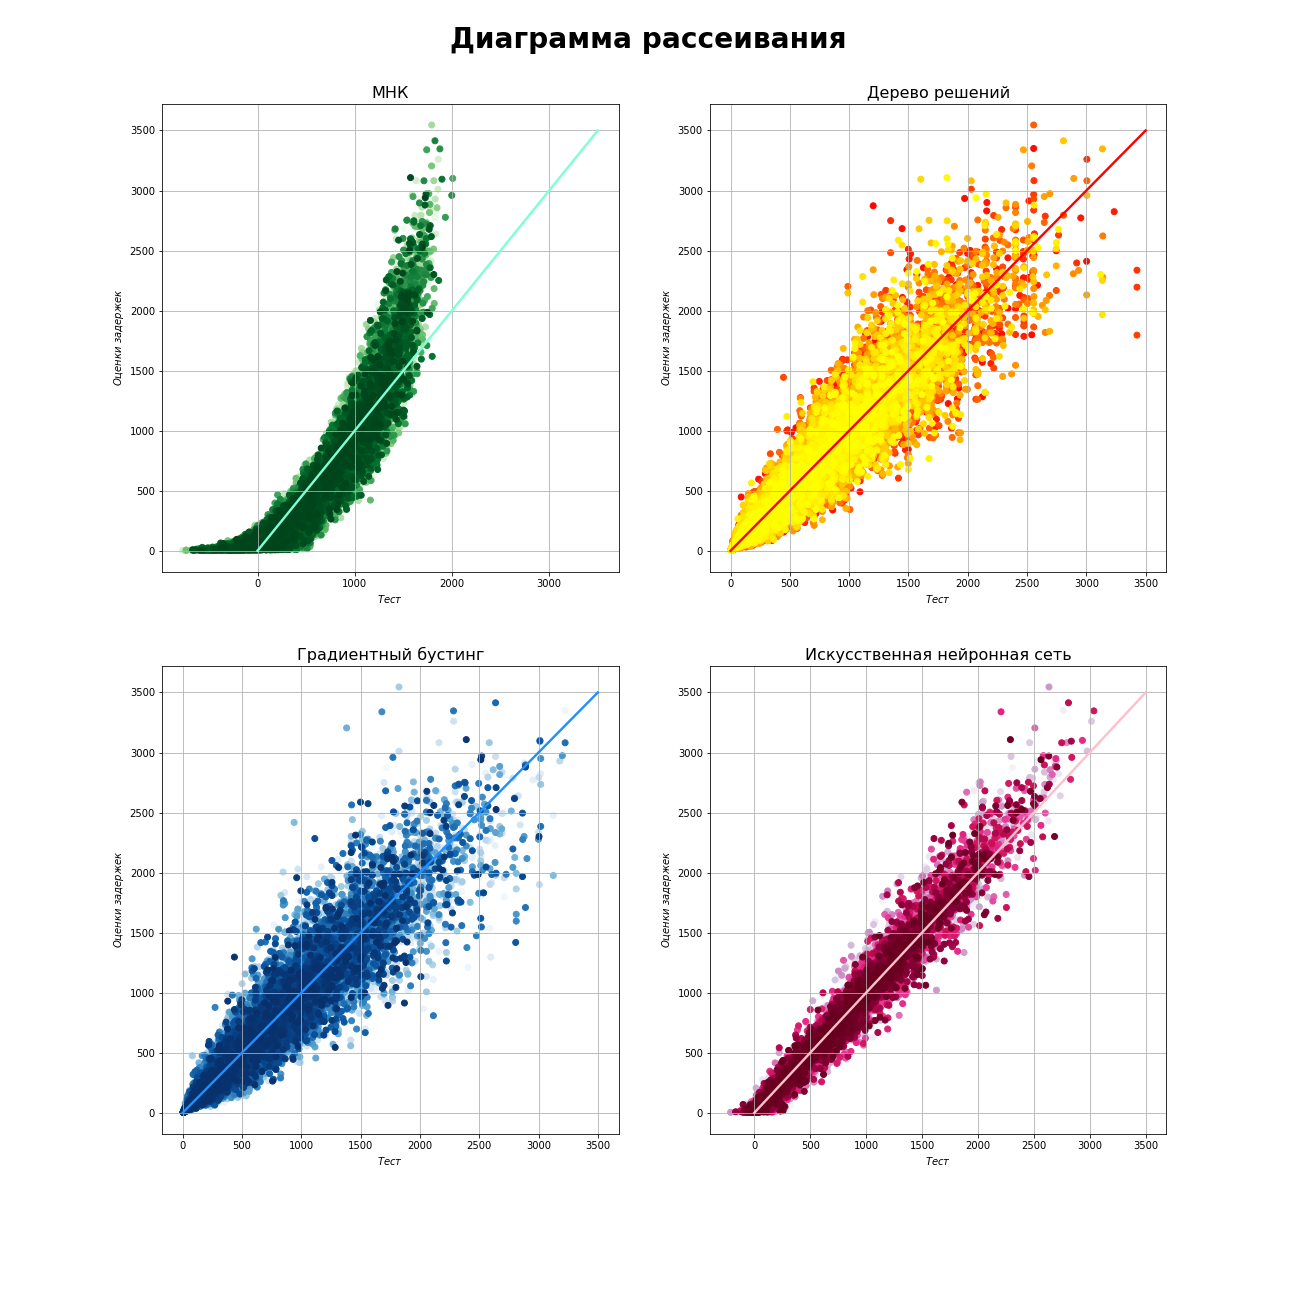
\includegraphics[width=0.95\textwidth]{total_scatter_diagram.png}
        \center{\textbf{Диаграмма рассеивания полученных моделей}}
        \bigskip
        \bigskip

    \end{minipage}

\end{frame}
    
\begin{frame}
    \justifying

    \fontsize{8pt}{7.2}\selectfont
    \center{\textbf{ Метрики моделей}}

    \begin{table}[b]\label{tab:total_reg_metrics}
        % \caption{ Метрики моделей}
        \begin{tabular}{|c|ccc|}
            \toprule
            Регрессионные модели    &$R$    & $STD$    &   $MAPE$\\
        
            \midrule
            \textbf{Метод наименьших квадратов} & 0,93   &   210,47  &   23,02 \\
            \textbf{Дерево решений} & 0.95   &   161,19  &   2,14 \\
            \textbf{Градиентный бустинг} & 0.952   &   165,04  &   2,16  \\
            \textbf{Искусственные нейронные сети} & 0.998   &   83,59  &   3,14  \\
            \bottomrule
        \end{tabular}
    \end{table}

    \center{\textbf{Оценка времени счета моделей межконцевой задержки на примере данных объемом 360.}}
    \begin{table}
        
        \begin{tabular}{|cc|}
            \toprule
            \textbf{Модель} & \textbf{Расчетное время, сек} \\
            \toprule
            Имитационная Модель & 172.2 \\
            МНК & $4.77\cdot 10^{-6}$  \\
            Деревья Решений & $5.48\cdot 10^{-6}$ \\
            Градиентный Бустинг & $5.01\cdot 10^{-6}$  \\
            Искусственные Нейронные Сети & $5.72\cdot 10^{-6}$ \\
    
    
            \bottomrule
        \end{tabular}
    \end{table}
\end{frame}

\begin{frame}
    \frametitle{Выводы по Положению 5}
    \fontsize{8pt}{7.2}\selectfont

    \textbf{Представлены:}
    \begin{itemize}
        \item построена имитационная модель СеМО;
        \item построены регрессионные модели с помощью методов машинного обучения для оценки времени межконцевой задержки сети.
    \end{itemize}

    \bigskip
    \textbf{Публикации:}
    \begin{minipage}[c]{1\linewidth}
        \fontsize{6pt}{7.2}\selectfont
        \begin{enumerate}
            \item \textit{Лазарева,В. Е.Расчёт межконцевых задержек и длин очередей вмногошаговой тандемной сети с применением методов машинногообучения [текст] / В. Е. Лазарева, А. А. Ларионов, А. А. Мухтаров //Материалы Всероссийской конференции с международным уча­стием "Информационно-телекоммуникационные технологии и мате­матическое моделирование высокотехнологичных систем"(Москва,2020). — 2020. — с. 43—48.20
            }.
        \end{enumerate}
    \end{minipage}

\end{frame}

% \section{Выводы}
\begin{frame}
    \frametitle{Выводы}
    
    \begin{enumerate}
        \item разработаны математические модели в виде экстремальной комбинаторной задачи и
        задачи ЦЛП для оптимального размещения базовых станций при
        проектировании беспроводных широкополосных сетей (БШС) с линейной топологией;
        \item предложен специальный алгоритм МВ и Г для решения сформулированной
        экстремальной комбинаторной задачи;
        \item разработана итерационная процедура нахождения последовательности лучших
        решений для задачи размещения базовых станций в рамках комплексного
        проектирования БШС с линейной топологией;
        \item разработаны математические модели для задач проектирования БШС с ячеистой
        топологией;
        \item предложены модели прогнозирования оценок характеристик производительности сети с
        помощью методов машинного обучения для многофазной сети массового обслуживания.
    \end{enumerate}
\end{frame}

% \section{Публикации}
\begin{frame}
    \frametitle{Публикации}
    \fontsize{8pt}{7.2}\selectfont

    Основные результаты по теме диссертации изложены в 12 печатных изданиях, 1 из которых издана в журнале, рекомендованных ВАК, 2 — в периодических научных журналах, индексируемых Web of Science и Scopus, 9 — в сборниках трудов конференции. 
    
    \bigskip
    
    В изданиях из списка \textbf{ВАК} 
    \begin{enumerate}
        \item \textit{Иванов,Р. Е.Задача оптимального размещения заданного множе­ства базовых станций беспроводной сети связи с линейной топо­логией [текст] / Р. Е. Иванов, А. А. Мухтаров, О. Першин //Автоматизация, телемеханизация и связь в нефтяной промышлен­ности. — 2019. — т. 549, No 4. — с. 39—45.}
    \end{enumerate}

    \bigskip

    В изданиях, входящих в международную базу цитирования \textbf{WoS и Scopus}

    \begin{enumerate}
        \item \textit{Ivanov,R.A Problem of Optimal Location of Given Set of Base Sta­tions in Wireless Networks with Linear Topology[текст]/ R. Ivanov,A. Mukhtarov, O. Pershin // Communications in Computer and Infor­mation Science. –– 2019. –– Vol. 1141 CCIS. –– P. 53––64. –– (Scopus,WoS).}
        \item  \textit{On Optimal Placement of Base Stations in Wireless Broadband Net­works to Control a Linear Section with End-to-End Delay Limited[текст]/ A. Mukhtarov [et al.] // Communications in Computer andInformation Science. –– 2020. –– Vol. 1337. –– P. 30––42.}
    \end{enumerate}

    \bigskip

    Все работы выполнены при финансовой поддержке Российского фонда фундаментальных исследований грант \textnumero{19-07-00919}.
\end{frame}

\begin{frame}
    \frametitle{Апробация работы}
    \begin{enumerate} % https://tex.stackexchange.com/a/476052/104425
        \fontsize{8pt}{7.2}\selectfont
        \item «Губкинский университет в решении вопросов нефтегазовой отрасли России» (Москва, 17-21 сентября 2018); 
        \item «13-е Всероссийское совещание по проблемам управления» (Москва, 17-20 июня 2019); 
        \item «International Conference on Distributed Computer and Communication Networks: Control, Computation, Communications» (Москва, 22-27 сентября 2019), 
        \item «Губкинский университет в решении вопросов нефтегазовой отрасли России» (Москва, 24-26 сентября 2019); 
        \item «Conference Management of Large-Scale System Development» (Москва, 1-3 октября 2019); 
        \item «Information and Telecommunication Technologies and Mathematical Modeling of High-Tech Systems» (Москва, 13-17 апреля 2020); 
        \item «Computer-aided technologies in applied mathematics» (Томск, сентябрь 2020);
        \item «International Conference on Distributed Computer and Communication Networks: Control, Computation, Communications» (Москва, 14-18 сентября 2020); 
        \item «Information and Telecommunication Technologies and Mathematical Modeling of High-Tech Systems» (Москва, 19-23 апреля 2021);
      \end{enumerate}
\end{frame}

\begin{frame}
    \frametitle{Положения}
    \begin{enumerate} % https://tex.stackexchange.com/a/476052/104425
        \item математические модели в виде экстремальной комбинаторной задачи и
        задачи ЦЛП для оптимального размещения базовых станций при
        проектировании беспроводных широкополосных сетей (БШС) с линейной топологией;
        \item специальный алгоритм МВ и Г для решения сформулированной
        экстремальной комбинаторной задачи;
        \item итерационная процедура нахождения последовательности лучших
        решений для задачи размещения базовых станций в рамках комплексного
        проектирования БШС с линейной топологией;
        \item математические модели для задач проектирования БШС с ячеистой
        топологией;
        \item модели прогнозирования оценок характеристик производительности сети с
        помощью методов машинного обучения для многофазной сети массового обслуживания.
      \end{enumerate}
\end{frame}

